\section{Introduction}
Platforms are becoming more and more significant in robotics. The two sorts of platforms are software platforms and hardware platforms. Low-level device control, SLAM (Simultaneous Localization and Mapping), navigation, manipulation, object or person recognition, sensing and package management, debugging and development tools are just a few of the characteristics that make up robot software platforms. These features are mostly used in the industrial sector, where robot software platforms are currently used most frequently. Robot hardware platforms include both industrial products and research platforms including humanoids, drones, and mobile robots. As a result, robotics researchers from around the world are working together to develop an open-source, user-friendly platform. Robot Operating System, sometimes known as ROS, is the most widely used robot software platform. The Robot Operating System, or ROS, is an open source framework for controlling the actions, motions, and other aspects of robots. In addition to those who have just started using robots, ROS is designed to be a software platform for both those who regularly develop and use robots.
\begin{figure}[H]
    \centering
    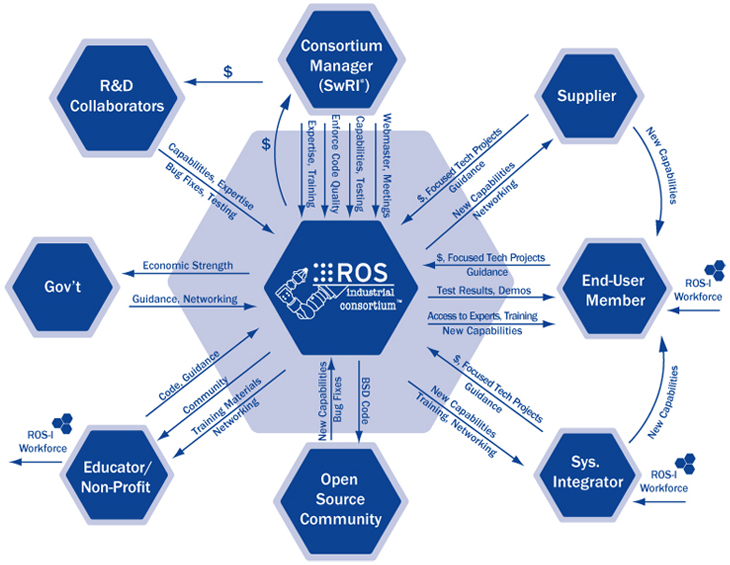
\includegraphics[scale=0.35]{Images/Chapter 2/ros_consortium.jpg}
    \caption{ROS Industrial Consortium}
    \label{fig:ros_consortium}
\end{figure}
\newpage
\section{History of ROS}
In the 1970s, the first specialized programming languages for robots emerged.
Robot-specific data types and libraries of robot functions existed. They did not permit integrated simulation, multi-robot interaction, or hardware abstraction. Standardization and code reuse were nonexistent.
Through the 1980s, 1990s, and particularly in the 2000s, when there was a strong drive to standardize robot components, their interfaces, and their fundamental functions, efforts to develop robot programming systems persisted.
\\
ROS was therefore first created in 2007 at the Stanford Artificial Intelligence Laboratory, where it is still used today. It has been controlled by OSRF since 2013, and it is now utilized by numerous robots, academic institutions, and businesses, becoming the de facto norm for robot programming.

% \begin{figure}[H]
%     \centering
%     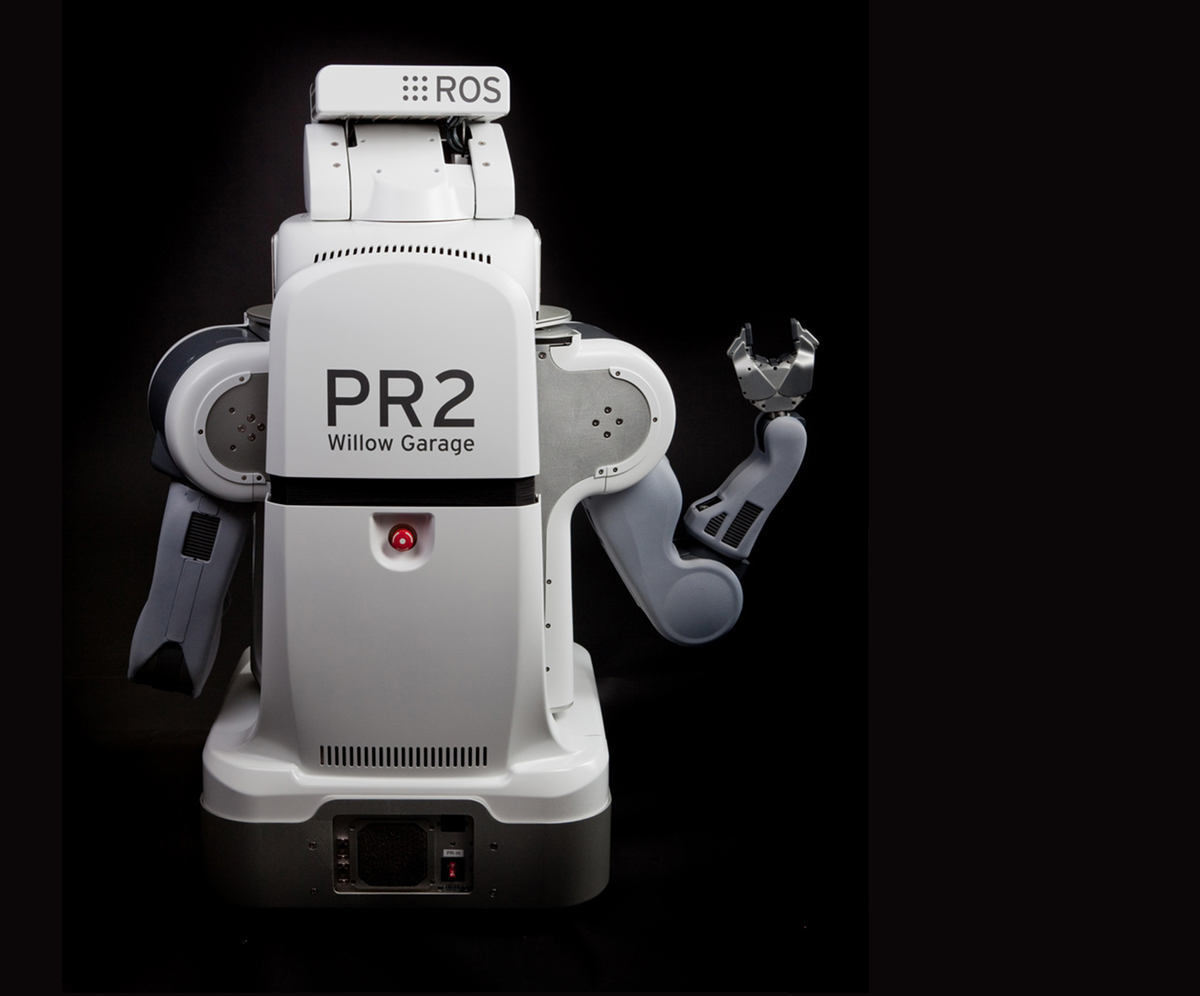
\includegraphics[scale=0.16]{Images/Chapter 2/PR2_Robot_Willow_Garage_6-1.jpeg}
%     \caption{Willow Garage PR2 robot}
%     \label{fig:PR2}
% \end{figure}
\section{Meta-Operating System}
ROS is merely a middleware because it is an open source, robot-specific operating system.
A middleware is a piece of software that acts as a layer between the operating system and the applications, providing the developer with an additional degree of abstraction.
It simply acts as a mediator between software parts, allowing for easier communication.
Its function is to give an abstraction model for functions and the low-level implementation at the same time.
Each middleware product must offer:
\begin{itemize}
    \item Portability: common programming model regardless the programming language and system architecture
    \item Complexity management: low-level aspects are managed by libraries and drivers inside the middleware itslef
    \item Reliability: middleware allows robot developer to discard low level details
    \item Abstraction from sensors/actuators hardware;
    \item Communication protocol for data transport
\end{itemize}
 As a result, they are crucial to the creation of sophisticated programs that rely on a variety of hardware and software resources. \\
They still need to go through a lot of development before they can offer a full range of capabilities for general-purpose robots.
 
\begin{figure}[H]
    \centering
    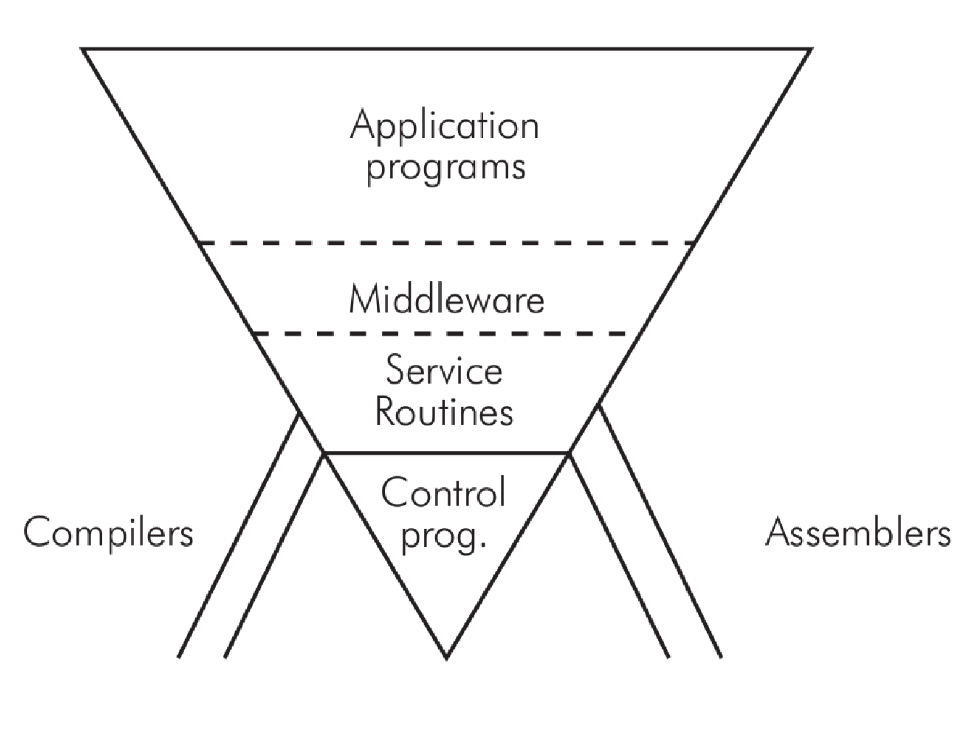
\includegraphics[scale=0.5]{Images/Chapter 2/middleware.png}
    \caption{Meta Operating System}
    \label{fig:metaoperating}
\end{figure}
 In recent years, a number of robotic middlewares (OROCOS, ORCA, YARP, BRICS, etc.) were put forth; eventually, ROS emerged. 

 \subsection{Phylosophy of ROS}
Some philosophical facets of ROS are described in the following sentences:\\
\begin{itemize}
\item \textit{Peer to peer}: ROS systems are composed of a small number of interconnected computer applications that are continuously exchanging messages. These communications flow directly between programs. The system becomes more complex as a result, but as the amount of data grows, the system balances better.\\
\item \textit{Distributed}: Programs can be run on multiple computers and comunicate over the network.
\item \textit{Multilingual}: ROS decided on a multilingual strategy. Any language that has a client library created for it can be used to create ROS software modules. Client libraries are available for C++, Python, LISP, Java, JavaScript, MATLAB, and other programming languages as of this writing. \\
\item \textit{Thin}: contributors are encouraged to build standalone libraries by the ROS conventions. and then wrap those libraries, so that they can send and receive messages to and from other ROS modules. This additional layer is proposed to allow the reuse of software developed outside of ROS for other applications, and it greatly simplifies the development of automated tests using standard continuous integration tools..\\
\item \textit{Free and open source}: Free and open source: The permissive BSD license is used to release the ROS core, which allows both commercial and non-commercial use. ROS foresees data exchange between modules using inter-process communication (IPC), which means that systems built using ROS can have fine-grained licensing of their various components.\\
\end{itemize}

\section{ROS Architecture}
Based on a graph architecture, ROS allows for processing to occur in nodes, which exchange messages with one another synchronously by calling services, much like RPCs, and asynchronously by using topics to which they can subscribe and/or publish. In terms of structure, ROS is created on three conceptual levels:
\begin{enumerate}
    \item File-system level
    \item Computational level
    \item Community level
\end{enumerate}
We'll look at each level's individual components and how they fit into the architecture.
\begin{figure}[H]
    \centering
    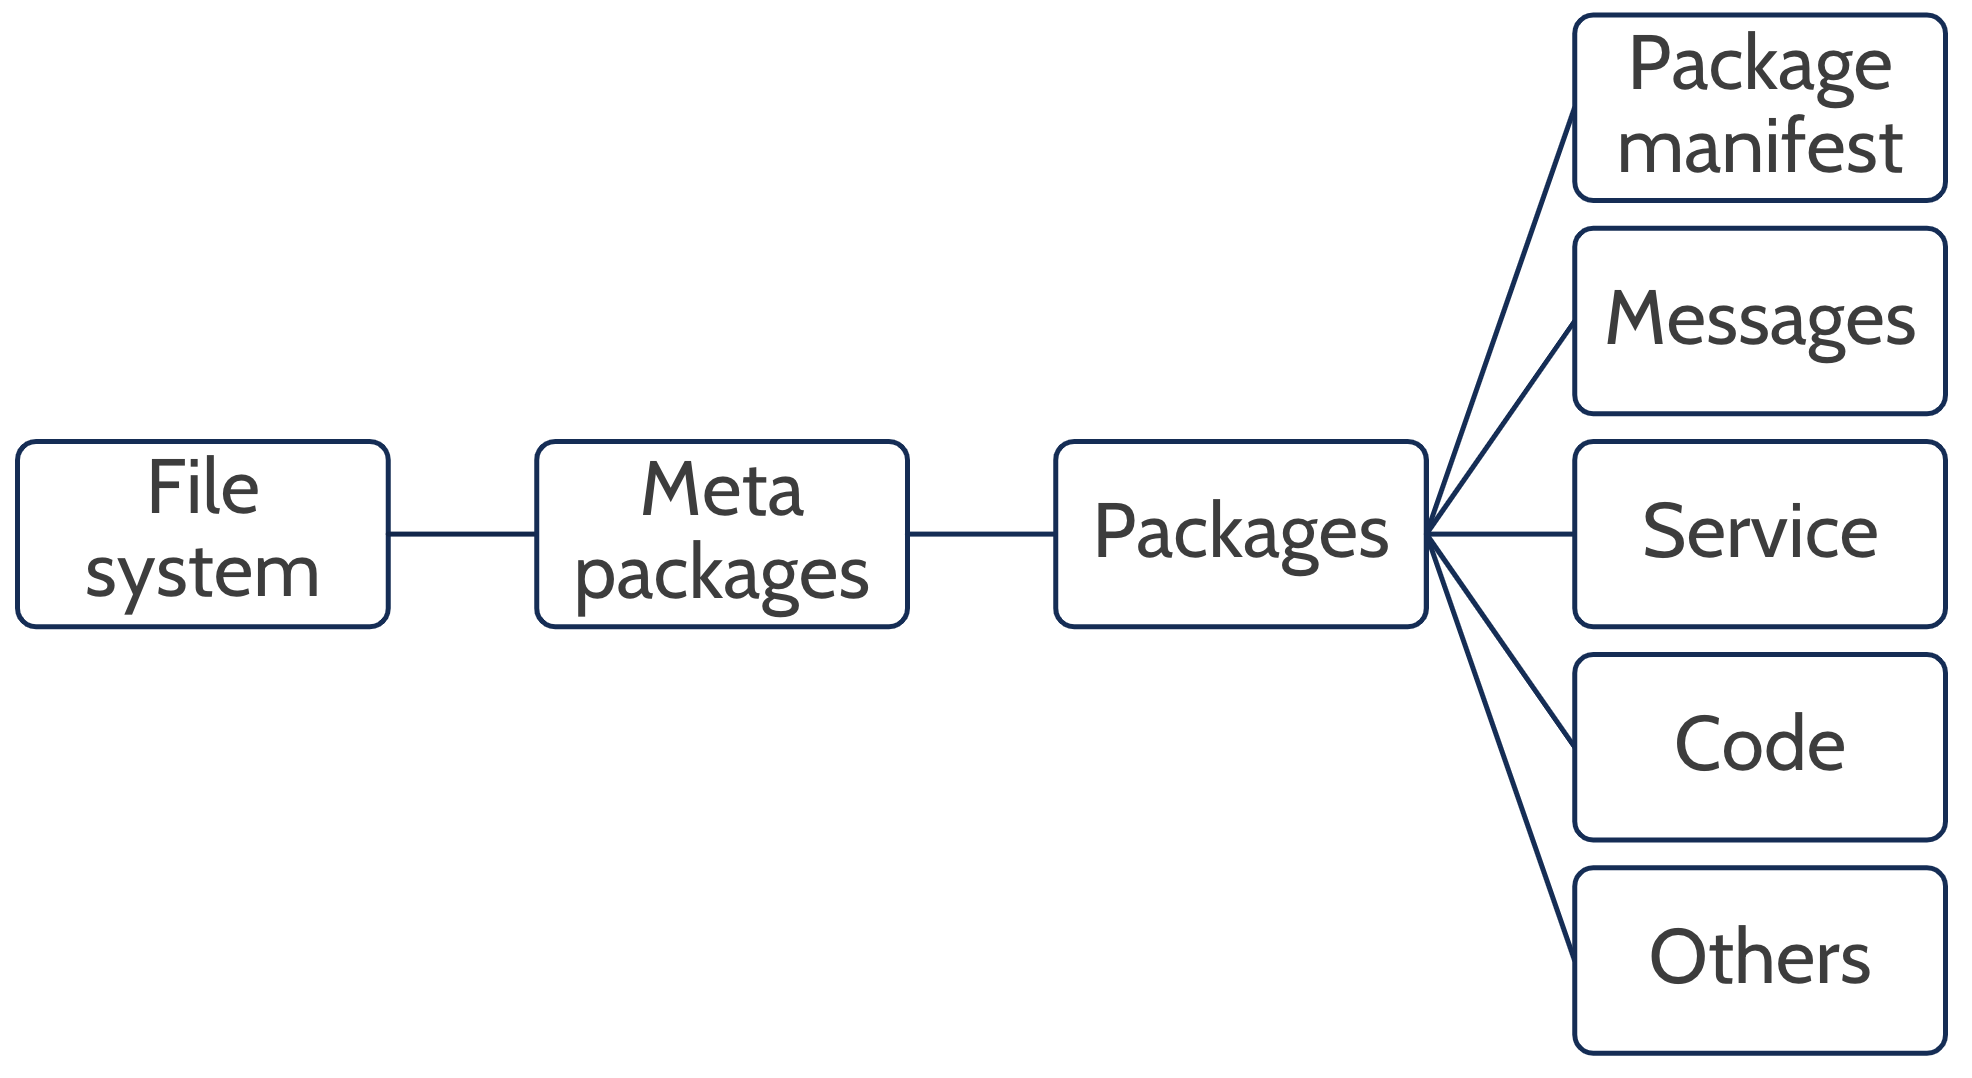
\includegraphics[scale=0.35]{Images/Chapter 2/Filesystem.png}
    \caption{File System level representation}
    \label{fig:Filesystem}
\end{figure}
\subsection{File-system Level}
The Filesystem Level includes all resources used in ROS, in particular
\begin{itemize}
    \item Packages
    \item Metapackages
    \item Manifest
    \item Message types
    \item Service types
\end{itemize}

\textbf{Packages}\\
Packages are the main structure for organising ROS, \citet{rospackages}. These files include all of the data needed by the system during runtime, including processes, libraries, configuration files, datasets, and other files. They make up the structural elements of a ROS-based system. The package is represented by a directory at the filesystem level. 

There are some subfolders within the framework to manage the elements in order to encourage its growth:
\begin{itemize}
    \item \textit{include/packagename}: C++ include headers (make sure to export in the CMakeLists.txt)
    \item \textit{msg}:Folder containing Message (msg) types
    \item \textit{src/packagename}: Source files, especially Python source that are exported to other packages.
    \item \textit{srv/}: Folder containing Service (srv) types
    \item \textit{scripts}: executable scripts
    \item \textit{CMakeLists.txt}: CMake build file
    \item \textit{package.xml}:XML file containing package structure 
    \item \textit{CHANGELOG.rst}: Many packages will define a changelog which can be automatically injected into binary packaging and into the wiki page for the package
\end{itemize}
\textbf{Metapackages}
Metapackages are specialised structures whose only task is to represent a group of packages that have common characteristics with each other. The metapackages that are created in the context of older versions of ROS and later updated may also result from the conversion of older stacks that perform similar functions in the context of older versions of ROS, \citet{rosmetapackages}.\\
\newline
\textbf{Manifest}\\
A package manifest consists of an XML file named package.xml that must be included in the root folder of any catkin-compliant package. It contains information about the package, including its name, version number, authors, maintainers, and dependencies on other catkin packages. There is a strong similarity between this concept and the manifest.xml file used in the legacy rosbuild build system. System package dependencies are declared in package.xml, \citet{rosmanifest}.\\
There are a minimal set of tags that need to be nested within the <package> tag to make the package manifest complete.
\begin{itemize}
    \item \textit{<name>}: The name of the package
    \item \textit{<version>}: The version number of the package;
    \item \textit{<description>}: A description of the package contents;
    \item \textit{<maintainer>}: The name of the person(s) that is/are maintaining the package;
    \item \textit{<license}: The software license under which the code is released.
\end{itemize}
\textbf{Message types}\\
Message types define the structure of messages sent by ROS, \citet{rosmsg}. A separate sort of message is represented by each file with the.msg extension. Each line in the file corresponds to a message field. Each line has two columns: one for the field's data type (Int32/int (C++/Phyton), bool, string, time, etc.), and the other for the field name. The fields contained within these le can have values assigned to them; in this case, we're talking about constants. Msg file example in C++:

\textbf{Service types}\\
Service type are files that define the structure of request/response for ROS services, \citet{rossrv}.
These directly build on the msg format to allow node-to-node communication. They are kept in specialized.srv files in a package's srv/ subdirectory.
Srv file example in C++:
\begin{minted}{cpp}
 bool add(beginner_tutorials::AddTwoInts::Request  &req,
             beginner_tutorials::AddTwoInts::Response &res)
    {
      res.sum = req.a + req.b;
      ROS_INFO("request: x=%ld, y=%ld", (long int)req.a, (long int)req.b);
      ROS_INFO("sending back response: [%ld]", (long int)res.sum);
     return true;
   }
\end{minted}

\subsection{ROS Computational Graph Level}
The peer-to-peer network of ROS processes that are working together to process data is known as the Computation Graph. Nodes, Master, Parameter Server, messages, services, topics, and bags are the fundamental Computation Graph concepts of ROS. Each of these components provides data to the Graph in a different manner, \citet{rosconcepts}.\\
\begin{figure}[H]
    \centering
    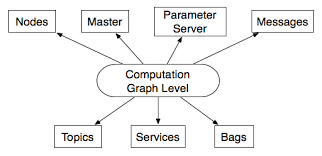
\includegraphics[scale=0.8]{Images/Chapter 2/computationgraph.png}
    \caption{Computation Graph}
    \label{fig:computationgraph}
\end{figure}
\textbf{Nodes}\\
A node is a process that performs computation. Nodes are combined together into a graph and communicate with one another using streaming topics, RPC services, and the Parameter Server, \citet{rosnodes}. In accordance with the concept of modularity of the system, each node will be connected to just one specific functionality. In order to make the system more reusable, manageable, and understandable, ROS actually discourages the development of "omnipotent" nodes that can do several tasks. \\
The utilization of nodes in ROS has several advantages for the entire system. Since crashes only affect certain nodes, there is more fault tolerance. Compared to monolithic systems, code complexity is decreased. \\

\textbf{Topics}\\
 The buses that enable message exchange between nodes are known as topics and have formal and distinctive names. They implement a method for publishing and subscribing, where nodes that are configured to transmit or receive messages can act as publishers or subscribers. Anonymity policies between the nodes clearly distinguish between data producers and users. A limit amount of messages for each topic may be maintained in the queue in case they accumulate; any extra messages are not added to the queue and are lost, \citet{rostopics}.\\
\newline
\textbf{Services}\\
A two-way communication tool between nodes is services. It is a method that expands on messages by giving users the option to continue listening to a particular node while also issuing commands to it in order to receive a structured response. Each service is initially documented in an.srv file, which also lists the arguments and the type of return data in addition to the name of the service.
The service is represented within the server node by a function that accepts two pointers to objects of the server class as inputs: one will contain the function parameters (Request), and the other will gather the return value, \citet{rosservice}\\
\newline
\textbf{Messages}\\
The nodes of the graph exchange messages in order to communicate. These could be straightforward primitive types (such as integer, string, char, etc.) or arrays, or they could be even more complex, with structures resembling those used in C.\\
\newline
\textbf{Bags}\\
The method through which ROS stores logs and keeps track of all communications exchanged within a subject is represented by bags. Once a topic has been assigned to the rosbag tool, every message that is exchanged is saved in a corresponding file with the.bag extension. It is highly helpful for storing sensor data because it enables the developer to make a sort of "black box" for the robot. Additionally, ROS has a playback tool that enables graphical interface playback and visualization of the acquired data.\\

\textbf{Master}\\
In ROS, the master is in charge of several tasks, including adding new nodes to the network, managing the connections among the nodes in the graph, routing messages, and allowing a node to access the services of another.
It is the brain of the program and can only be used by one master concurrently. If the file is implemented properly, it can be started using the roscore command or launched automatically when a node starts.
\begin{figure}[H]
    \centering
    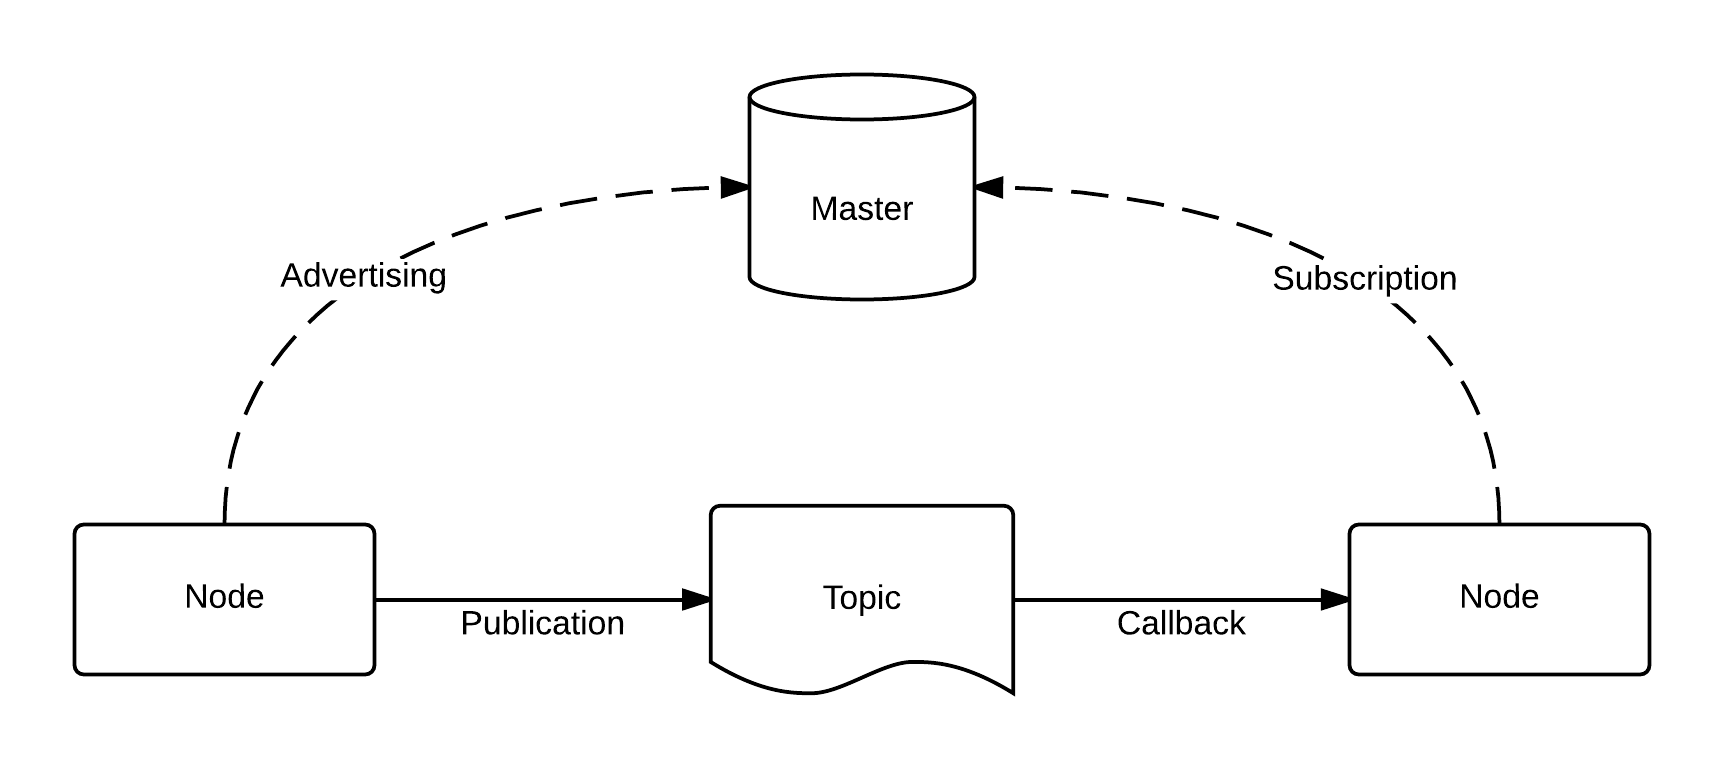
\includegraphics{Images/Chapter 2/ROS-master-node-topic.png}
    \caption{Visualization of Master-Node-Topic relationship}
    \label{fig:master-node-topic}
\end{figure}

\textbf{Parameter server}\\
The parameter server is essentially a component of the master, allowing certain network API configurations to be shared publicly with all nodes. Although not particularly fast, it is still useful during the software testing phase. The parameters are named according to the standard ROS naming convention. This means that ROS parameters follow the same hierarchical structure as topics and nodes, \citet{rosparmserv}.

\subsubsection{Coordinate Frames and Transforms}
A robot typically has numerous 3D reference systems that change over time. All of these coordinate systems are kept in a tree structure by the ROS tf package. This concept is also required to understand how URDF files handle the various parent and child links later on. As a result, the tf package keeps track of all existing relationships between point co-ordinate frames and calculates transforms between them. Developers can also use the command view frames to view the transform tree for debugging purposes.

\begin{figure}[H]
    \centering
    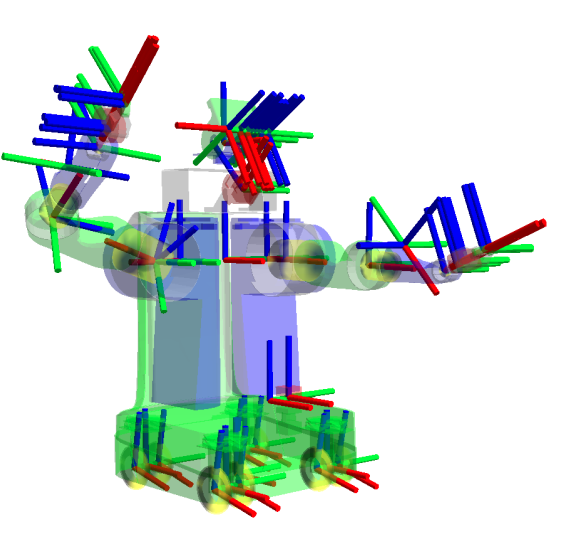
\includegraphics[scale = 0.5]{Images/Chapter 2/robottf.png}
    \caption{Transform Frames of a robot}
    \label{fig:robottf}
\end{figure}

\begin{figure}[H]
    \centering
    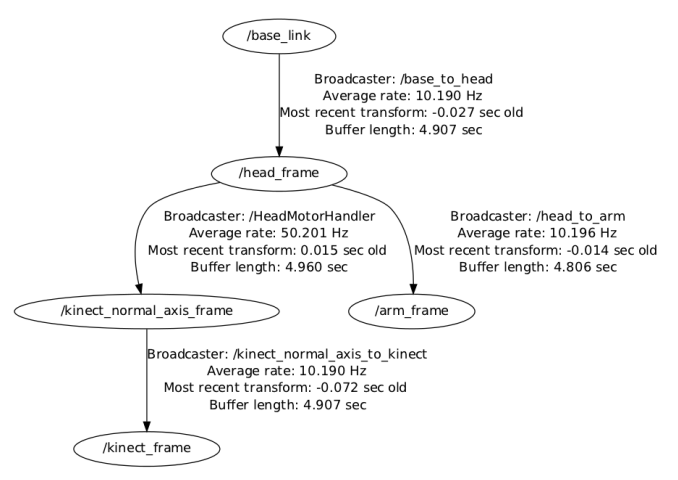
\includegraphics[scale = 0.5]{Images/Chapter 2/robottftree.png}
    \caption{Transform Frames Tree of a robot}
    \label{fig:robottf}
\end{figure}
\section{ROS Tools and Simulators}
ROS includes built-in tools that can be used when developing robotic applications or delving deeper into certain issues.
Although other tools exist, the ones described below were the ones that were used the most during the Oversonic project: RViz (3D visualization tool), Rqt (framework that enables GUI tools: Rqt graph, which displays correlation between nodes and messages in graph form, and Rqt plot), and, finally, Gazebo, a 3D simulator that has long been used in the course of this project, will be highlighted.
\subsection{RViz: 3D Visualization Tool}
RViz is a 3D visualization tool built into ROS.
Its primary function is to visualize ROS messages and topics in three dimensions, assisting the user in displaying data and understanding how our system behaves.
When starting a new RViz window from scratch, a black 3D scene appears. The user can indeed customize the environment by changing global options (for example, the fixed frame that provides a static reference view) and grid settings.
It is possible to choose which features to display by ticking them directly from the left panel (picture \ref{fig:rvizgui}).
RViz can visualize topic from camera sensor, showing the images on a dedicated box. This feature applies to any kind of sensor that communicates via ROS to our robot, e.g. Lidar, tracking camera, RGB camera etc. 
\begin{figure}[H]
    \centering
    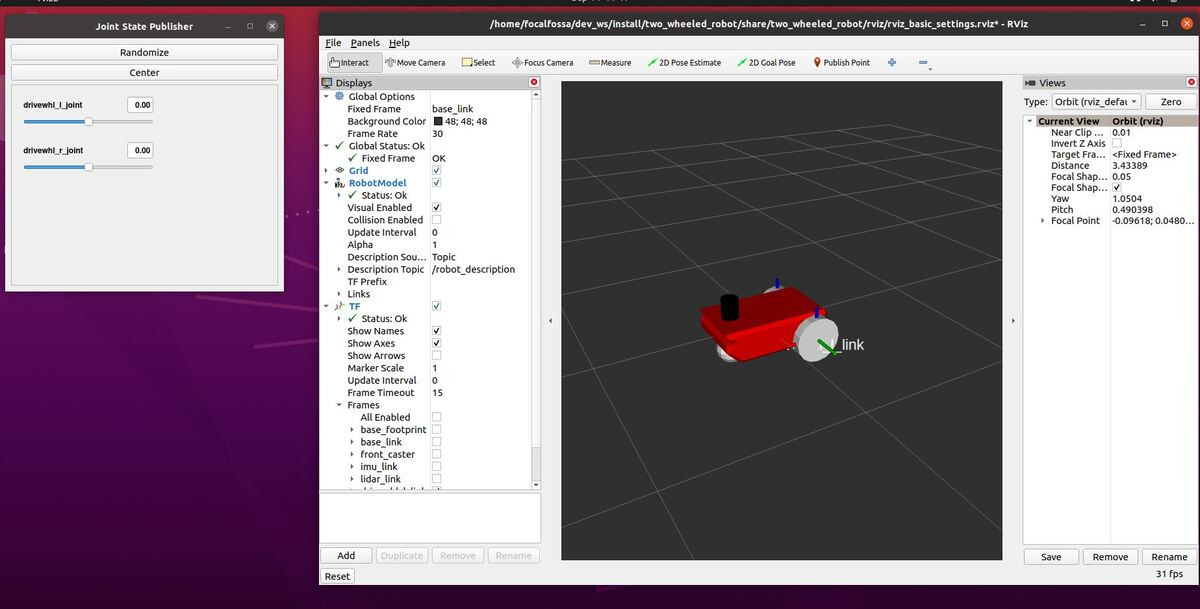
\includegraphics[scale = 0.5]{Images/Chapter 2/rviz.jpg}
    \caption{RViz GUI}
    \label{fig:rvizgui}
\end{figure}
\subsection{Rqt: ROS GUI Development Tool}
Rqt is a ROS software framework that implements various GUI tools as plugins.
Rqt graph, in particular, is extremely useful.
The primary goal of this tool is to visualize ROS nodes, topics, and messages to aid in debugging and understanding of the system. In fact, when using ROS, it is beneficial to display the current graph in order to better understand how the various nodes communicate and how messages are exchanged.
Rqt graph thus results useful in:
\begin{itemize}
    \item Having a global overview of the system
    \item Debugging code in case there exist issues in nodes communication (e.g. two nodes are not connected in reality or too many nodes publish on the same topic)
\end{itemize}
\begin{figure}[H]
    \centering
    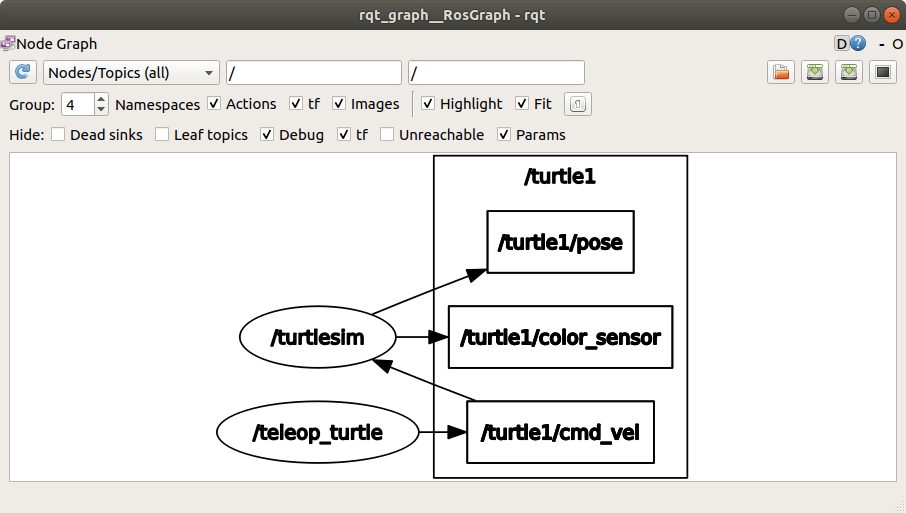
\includegraphics[scale=0.3]{Images/Chapter 2/rqt_graph_turtlesim.png}
    \caption{Graph from turtlesim}
    \label{fig:rqtgraph}
\end{figure}
In figure \ref{fig:rqtgraph} two nodes have been initialized and from the graph we can see the path of the messages.
 \subsection{Gazebo Simulator}
Dealing with real robots means using physics labs, charging batteries, calibrating sensors and many other small tasks involving hardware.
In real-life cases, even the best robots break down periodically due to human error, wear and tear or structural defects.  This is where simulators come in: in simulation, we can faithfully simulate the actions that the robot will perform, without the disadvantages listed above.
It is also possible to model actuators and sensors either as ideal devices or by adding varying degrees of distortion, error or failure. Thus, the solution of simulating robots in a virtual environment is efficient and cost effective.
The problem of SLAM (simultaneous localisation and mapping) has always been one of the most important research topics in the community.
In response to this need, 'Stages', for example, with high computational capabilities and different kinematic configurations, built-in sensors have been developed over the years.
In the context of this paper, it was decided to use Gazebo, a 3D simulator that provides various models of robots, sensors, environments, offering faithful and reliable simulations thanks to its physics engine. Gazebo is in fact one of the best-known simulators used in open source robotics.
 \begin{figure}[H]
     \centering
     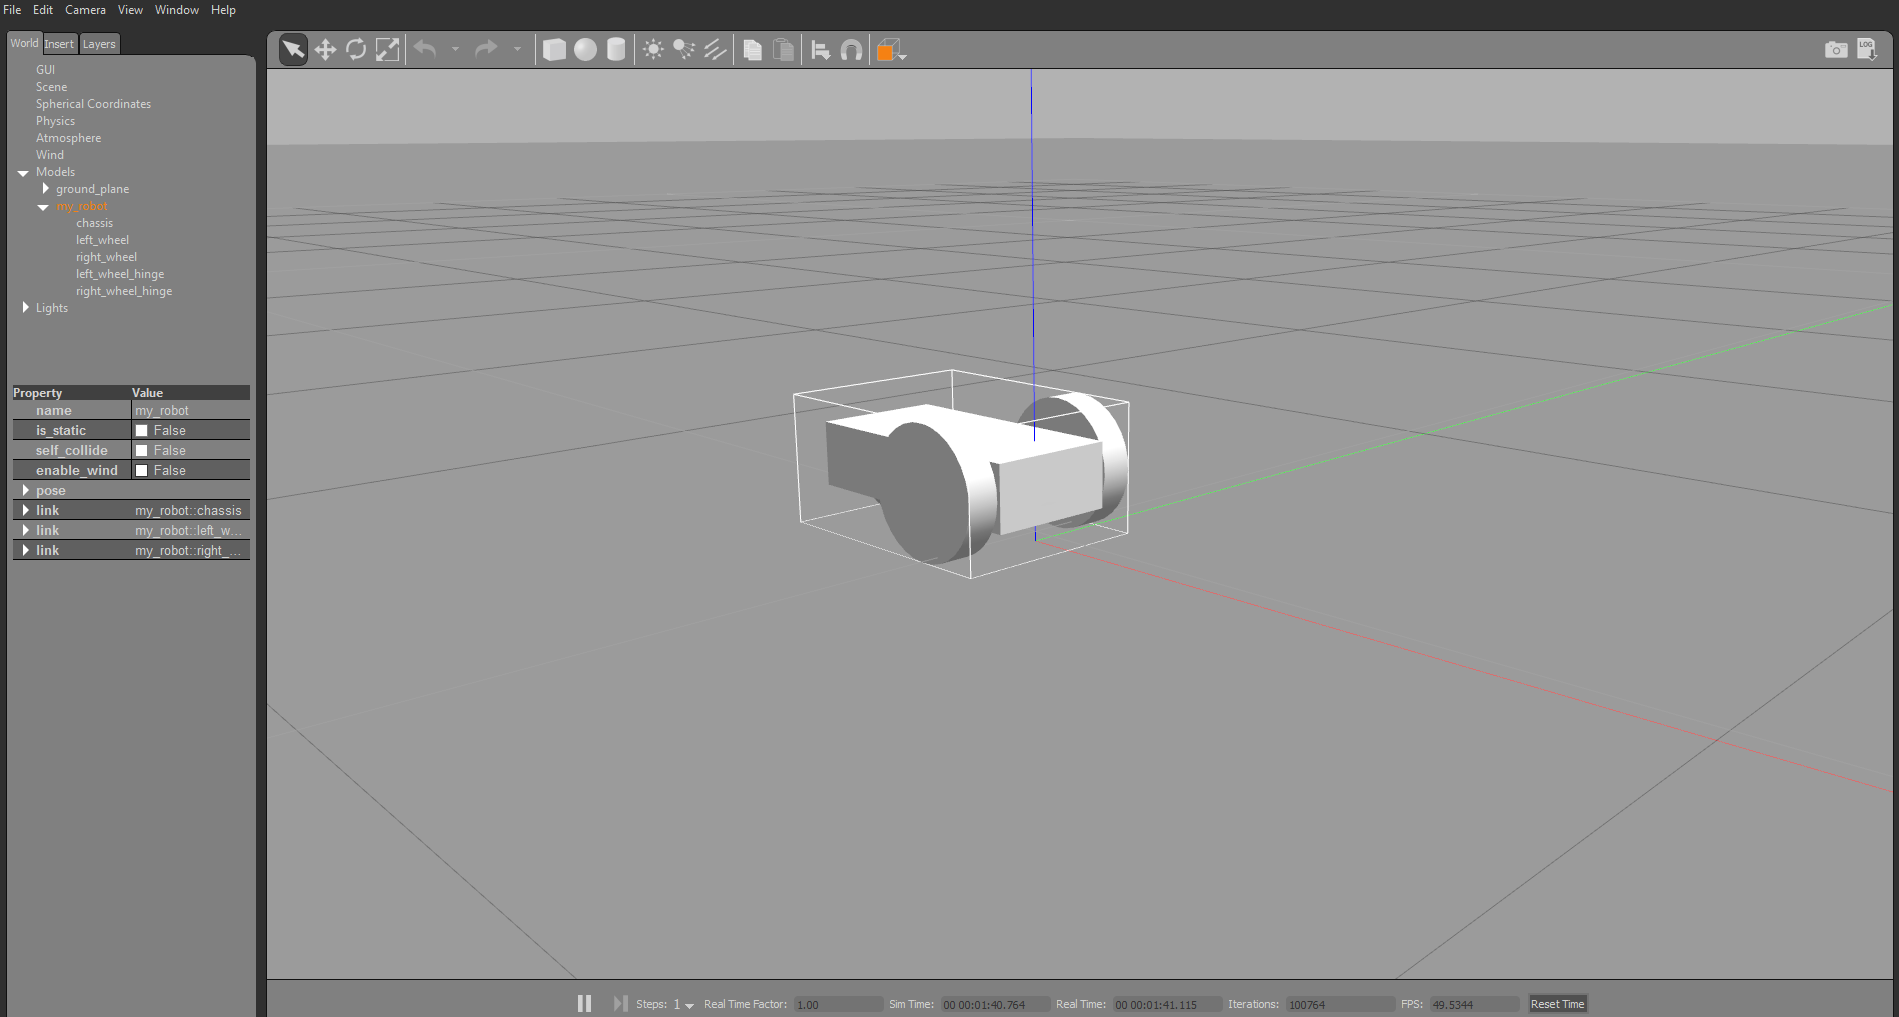
\includegraphics[scale=0.25]{Images/Chapter 2/gazebogui.png}
     \caption{Gazebo GUI}
     \label{fig:gazebogui}
 \end{figure}
To use the simulator, you can either download a pre-fabricated model from the Gazebo robots (such as TurtleBot, PR2, Pioneer2, and other well-known robots) or build your own robot model (we'll discuss SDF and URDF later).
In terms of robots, your model can be equipped with a variety of sensors, including a stereo camera, RGB camera, tracking, and contact sensors. The noise model can also be added to the sensors.
ROS is tightly integrated with Gazebo thanks to the gazebo ros package. This is a simulator plugin module that enables bi-directional communication between Gazebo and ROS.
Simulated sensors and physical simulation data are thus bidirectionally transmitted between the two platforms.
 \begin{figure}[H]
     \centering
     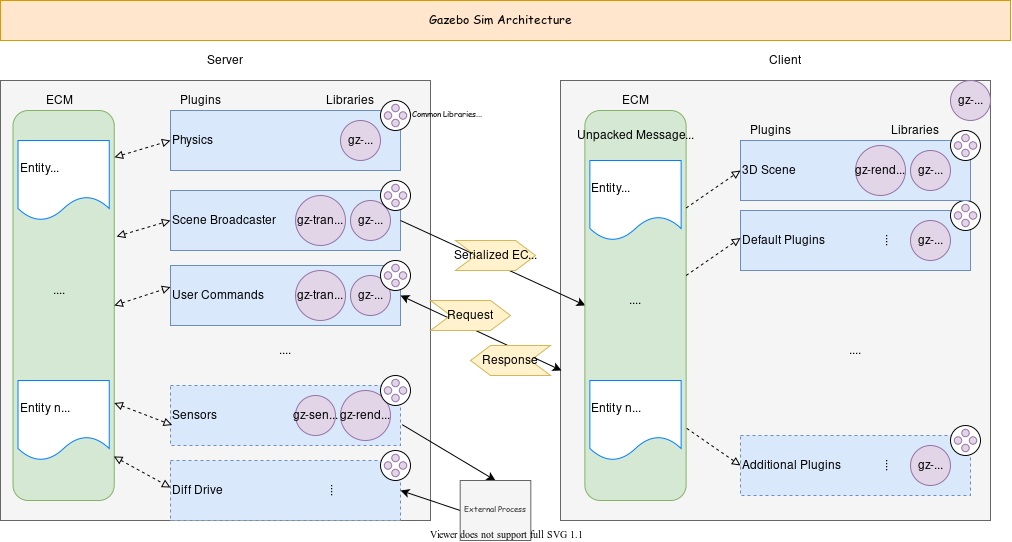
\includegraphics[scale=0.40]{Images/Chapter 2/GazeboSimArchitecture.png}
     \caption{Gazebo Sim Architecture}
     \label{fig:gazebosimarch}
 \end{figure}
 
\subsubsection{Robot Modelling Formats}
As mentioned above, one of the possible ways of describing a robot model is through the URDF.
The unified robot description format is a package containing a file in XML format.
A URDF file is written in such a way that each link of the robot is a child of some other parent link, with joints connecting each link. In turn, the joints are defined by an offset from the reference frame of the parent link and their axis of rotation. 
This creates a complete kinematics model. 
Below is reported a simple sample of the creation of a base link:
\begin{minted}{xml}
    <link name="base_link">
    <visual>
      <geometry>
        <cylinder length="0.6" radius="0.2"/>
      </geometry>
      <material name="blue"/>
    </visual>
    <collision>
      <geometry>
        <cylinder length="0.6" radius="0.2"/>
      </geometry>
    </collision>
    </link>
\end{minted}

When we are developing complex robot models, it can happen that the notation within the XML file becomes verbose and prone to confusion.
It is precisely for this reason that the XACRO (Macros XML) model was created, which is nothing more than an XML  that allows the design phase of the model to be divided into sub-parts, which are then imported one by one into the main file. 
This results in cleaner code reading and facilitates debugging.

Below is an example of importing arguments from an external file:
\begin{minted}{xml}
    <xacro:property name=”robotname” value=”R001” />
    <link name=”${robotname}s_leg” />
\end{minted}

To use the model created within the Gazebo environment (which, as previously stated, works with SDFormat files), first convert from XACRO to URDF and then from URDF to SDF. In fact, files in this format include a description of the world in which the robot will be placed, a number of simulated physical world features (static and dynamic objects, lighting, terrain, and even physics), and plug-in additions.
An SDF file defining a model from scratch is shown below.:

\begin{minted}{xml}
<?xml version='1.0'?>
<sdf version='1.9'>
  <model name='my_model'>
    ...
  </model>
</sdf>
\end{minted}





